\documentclass[12pt, letterpaper]{article}
\usepackage[utf8]{inputenc}
\usepackage{amsmath}
\usepackage{amsthm}
\usepackage{amssymb}
\usepackage{colortbl}
\usepackage[a4paper, total={6.5in, 10in}]{geometry}

\usepackage{graphicx}
\graphicspath{ {/} }
\newtheorem{problem}{Problema}
\title{Computación Concurrente - Tarea 1}
\author{Damián Rivera González\\Alexis Hernandez Castro}

\begin{document}
\maketitle
\begin{itemize}
\item[1. ] Considera un problema computacional que puede resolverse secuencialmente en tiempo $n^3$, por ejemplo operaciones en matrices cuadradas $n\times n$ y la unidad de tiempo es 1 nanosegundo ($10^{-9}$). Des esta manera, si $n = 1000$, el cómputo tomaría $1000^3 \times 1 ns = 1s$. Supón que has creado un algoritmo concurrente que trabaja de manera completamente eficiente, es decir, el cómputo total tarda $\frac{n^3}{p}$ ($p$ es el número de hilos). Qué tan grande es la entrada que se puede manejar en: 

\begin{itemize}
\item[a, a) ] Un segundo y 8 hilos
$$\frac{n^3}{8} = 1s$$
$$n^3 = 1s \times 8$$
$$n = \sqrt[3]{1s \times 8}$$
$$n = 2000$$

\item[a, b) ] Un segundo y 1000 hilos
$$\frac{n^3}{1000} = 1s$$
$$n^3 = 1s \times 1000$$
$$n = \sqrt[3]{1s \times 1000}$$
$$n = 10000$$

\item[a, c) ] Un segundo y 1000000 hilos
$$\frac{n^3}{1000000} = 1s$$
$$n^3 = 1s \times 1000000$$
$$n = \sqrt[3]{1s \times 1000000}$$
$$n = 100000$$

\item[b, a) ] Un minuto y 8 hilos
$$\frac{n^3}{8} = 60s$$
$$n^3 = 60s \times 8$$
$$n = \sqrt[3]{60s \times 8}$$
$$n = 7829.73$$

\item[b, b) ] Un minuto y 1000 hilos
$$\frac{n^3}{1000} = 60s$$
$$n^3 = 60s \times 1000$$
$$n = \sqrt[3]{60s \times 1000}$$
$$n = 39148.67$$

\item[b, c) ] Un minuto y 1000000 hilos
$$\frac{n^3}{1000000} = 60s$$
$$n^3 = 60s \times 1000000$$
$$n = \sqrt[3]{60s \times 1000000}$$
$$n = 391486.76$$

\item[c, a) ] Un mes y 8 hilos
$$\frac{n^3}{8} = 2592000s$$
$$n^3 = 2592000s \times 8$$
$$n = \sqrt[3]{2592000s \times 8}$$
$$n = 274731.41$$

\item[c, b) ] Un mes y 1000 hilos
$$\frac{n^3}{1000} = 2592000s$$
$$n^3 = 2592000s \times 1000$$
$$n = \sqrt[3]{2592000s \times 1000}$$
$$n = 1373657.09$$

\item[c, c) ] Un mes y 1000000 hilos
$$\frac{n^3}{1000000} = 2592000s$$
$$n^3 = 2592000s \times 1000000$$
$$n = \sqrt[3]{2592000s \times 1000000}$$
$$n = 13736570.91$$
\end{itemize}
¿Cuántos hilos se necesitan si se quisiera resolver un problema con $n = 10^6$ en un año? 

$$\frac{(10^6)^3}{p} = 31536000s$$
Despejando a $p$ tenemos:
$$p = \frac{1\times 10^{18}}{31536000s} = 31709791983\leftarrow hilos$$
\\
\item[2. ] Usa la ley de Amdahl para resolver las siguientes preguntas:
\begin{itemize}


	\item[a)]Sup\'on que un programa tiene un m\'etodo M que no puede ser paralelizado y que este m\'etodo cuenta el $45\%$ del tiempo de la ejecuci\'on del programa. ¿Cu\'al es el lım\'ite de speedup general que se puede lograr ejecutando el programa en una máquina con n procesos? \\
	
	Respuesta:\\ Usando la ley de Amdahl $\frac{1}{(1-p)+\frac{p}{n}}$ tenemos lo siguiente $\frac{1}{(1-.45)+\frac{.45}{n}}$ a esto le aplicamos el limite de cuando n tiende a infinito lo cual la seccion $\frac{.45}{n} = 0$ sustituyendo tenemos $\frac{1}{.55} = 1.88x$ \\
	
	\item[b)]{Sup\'on que el m\'etodo M cuenta el $35$ del tiempo de la ejecuci\'on del programa. Sea s n el speedup con n procesos. Tu jefe te dice que debes duplicar este speedup: la versión nueva del programa debe tener un speedup $s_{n}^{'} \geq 2 * s_{n} $. Tu buscas a un programador para reemplazar M con una version mejorada, k veces m\'as r\'apida. ¿Qu\'e valor de k es requerido?}\\

	Respuesta:\\
	Observaci\'on 1:$s_{n} = \frac{1}{1-.65 +\frac{.65}{n}}$ donde aplicamos el limine donde n tiende a infinito tenemos como resultado $s_{n} = 2.85$ \\

	Observaci\'on 2:$s_{n}^{'} \geq 2*2.857$ que es lo mismo que $\frac{1}{p^{'}} \geq 5.7$ despejando a $p^{'}$ tenemos que debe tener valores entre $.824 \leq p^{'} < 1 $\\

	Usando las observaci\'ones 1 y 2 tenemos que $s_{n}^{'} =  \frac{1}{(1-p)*k}$ donde k es la mejora del programa M sustituyendo tenemos que $5.68 = \frac{1}{(1-.65)*k}$ por lo tanto $K \approx.5030$\\
	
	\item[c)]{Sup\'on que el m\'etodo M se puede acelerar tres veces. ¿Qué fracci\'on de todo el tiempo de ejecuci\'on debe contar M para que se pueda doblar el speedup del programa?}\\
	
	Respuesta:\\
	Sabemos que otra intepretacion del speedup es $t^{'} = \frac{t}{s}$ donde t es el tiempo a mejorar y s es la aceleracionmejorada y $t^{'}$ es el tiempo que debe tomar. Sustituyemdo en esta interpretacion tenemos que $t^{'} = \frac{3x}{2x} = \frac{3}{2}$ que es la fraccion de tiempo que se debe mejorar para doblar el speedup del programa M.
	
\end{itemize}

\item[3. ]Al ejecutar tu aplicaci\'on con dos procesadores se produce un speedup $S_{2}$ . Utiliza la Ley de Amdahl para derivar una f\'ormula para $S_{n}$ (speedup con n procesadores), en t\'erminos de n y $S_{n}$ .\\
Respuesta:\\
Primero notemos que el speedup de 2 procesadores es $s_{2} = \frac{1}{(1-p)+\frac{p}{2}}$ y el speedup de n procesadores es $s_{n} = \frac{1}{(1-p)+ \frac{p}{n}}$ si despejamos a p en $s_{2}$ tenemos que $p = \frac{1-s_{2}}{s_{2}(\frac{1}{n}-1)}$\\
Ahora sustituimos p en $s_{n}$ factorizando y minimizando tenemos que $s_{n}=\frac{s_{2}}{n(s_{2}-1)+s_{2}}$
\item[4. ]Calcula el speedup que tendrı\'a un programa con 100 procesadores si al medir el programa en forma secuencial se tarda 188 segundos y con dos procesadores tarda 104 segundos.\\
Respuesta:\\
Observemos que usando la interpretacion de speedup de esta manera $S(n)=\frac{T_{seq}}{T_{par}(n)}$
tenemos que el speedup de dos procesadores en este ejemplo es:\\ 
$S(2) = \frac{188s}{104s} \approx 1.8076$ y ahora ocupamos la formula del ejercicio anterior que es: 
\begin{center}
$s_{n}=\frac{s_{2}}{n(s_{2}-1)+s_{2}}$ \\
\end{center}
Ahora sustituimos en la formula por lo que obtenemos:\\
$S(100) =\frac{1.8076}{100(1.8076-1)+1.8076}\approx 0.02189$ 

\item[5. ] Considera la siguiente clase que representa un contador:\\
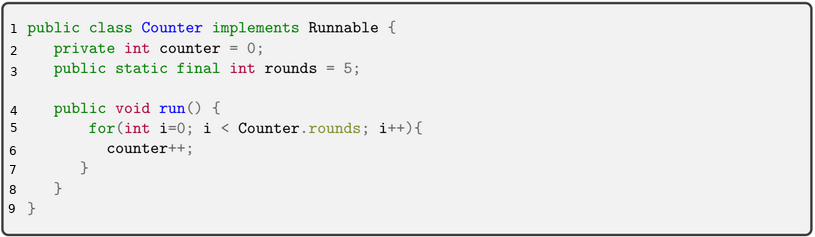
\includegraphics[width=\textwidth]{Codigo5}\\
Suponiendo que los hilos se ejecutan concurrentemente sobre el contador. Contesta las siguientes preguntas.
\begin{itemize}
\item[a) ] Demuestra que no existe una ejecución en donde el valor del contador sea 0.\\

Como sabemos, hay dos hilos, llamemosle $h1$ y $h2$, para los cuales sin importar cuantas iteraciones tengan en su ciclo $for$, la última instrucción que se lleva a cabo es $counter++$, por lo que al menos uno de los dos hilos, $h1$ o $h2$, terminará su ejecución con esta instrucción, y si en un inicio $counter = 0$, al final su valor será aumentado en una unidad. Por lo tanto el valor de $counter$ no puede terminar con valor 0. 

\item[b) ] Demuestra que no existe una ejecución en donde el valor del contador sea 1.

[Por contradicción] Sabemos que hay dos hilos, llamemosle $h1$ y $h2$. Supongamos que el valor del contador termina en 1. Como sabemos que cada hilo ejecuta el método $run$ en el cual la última instrucción es $counter++$, supongamos sin perdida de generalidad que el hilo $h2$ termina la útlima ejecución de $counter++$ significa que el $h2$ leyó $counter = 0$ teniendo así dos casos: 
\begin{itemize}
\item[Caso 1. ] Es la última iteración del $for$ en $h2$.\\
Lo cual implica que $h2$ leyó 5 veces a $counter = 0$, lo cual no se podría puesto que $h1$ ha terminado con todas sus iteraciones y al menos aumento en una unidad el valor de $counter$, por lo tanto $h2$ no pudo haber leido $counter = 0$.

\item[Caso 2. ] No es la última iteración del $for$ en $h2$.\\
Lo que significa que al menos $h2$ o $h1$ aumentaran en una unidad el valor de $counter$ por lo que $h2$ no podría terminar leyendo en la penúlitma acción a $counter = 0$.
\end{itemize} 

\item[c) ] Muestra una ejecución en donde el valor final del contador sea 2.\\
\resizebox*{.75\textwidth}{!}{
\begin{tabular}{|c | c | c|}
\hline
\rowcolor[gray]{0.9}$H1$ & $H2$ & Memoria \\
\hline 
PC 4 & PC 4 & counter = 0\\
PC 5, i = 0 & PC 5, i = 0 & counter = 0\\
PC 6, i = 0, read(counter)& PC 6, i = 0, read(counter) = 0 & counter = 0\\
PC 6, i = 1, write(counter++) & & counter = 1\\
PC 6, i = 1, read(counter)& & counter = 1\\
PC 6, i = 2, write(counter++) & & counter = 2\\
PC 6, i = 2, read(counter)& & counter = 2\\
PC 6, i = 3, write(counter++) & & counter = 3\\
PC 6, i = 3, read(counter)& & counter = 3\\
PC 6, i = 4, write(counter++)& & counter = 4\\
 & PC 6, i = 1, write(counter++) & counter = 1\\
PC 6, i = 4, read(counter)& PC 6, i = 1, read(counter) & counter = 1\\
 & PC 6, i = 2, write(counter++) & counter = 2\\
 & PC 6, i = 2, read(counter) & counter = 2\\
 & PC 6, i = 3, write(counter++) & counter = 3\\
 & PC 6, i = 3, read(counter) & counter = 3\\
 & PC 6, i = 4, write(counter++) & counter = 4\\
 & PC 6, i = 4, read(counter) & counter = 4\\
 & PC 6, i = 5, write(counter++) & counter = 5\\ 
PC 6, i = 5, write(counter++) & & counter = 2\\
\hline
\end{tabular}}\\

\item[d) ] Muestra una ejecución en donde el valor final del contador sea 7.\\
\resizebox*{.75\textwidth}{!}{
\begin{tabular}{|c | c | c|}
\hline
\rowcolor[gray]{0.9}$H1$ & $H2$ & Memoria \\
\hline 
PC 4 & PC 4 & counter = 0\\
PC 5, i = 0 & PC 5, i = 0 & counter = 0\\
PC 6, i = 0, read(counter)& PC 6, i = 0, read(counter) = 0 & counter = 0\\
PC 6, i = 1, write(counter++) & PC 6, i = 1, write(counter++) & counter = 1\\
PC 6, i = 1, read(counter)& PC 6, i = 1, read(counter) & counter = 1\\
PC 6, i = 2, write(counter++) & PC 6, i = 2, write(counter++) & counter = 2\\
PC 6, i = 2, read(counter)& & counter = 2\\
PC 6, i = 3, write(counter++) & & counter = 3\\
PC 6, i = 3, read(counter)& & counter = 3\\

PC 6, i = 4, write(counter++) & & counter = 4\\
PC 6, i = 4, read(counter)& PC 6, i = 2, read(counter) & counter = 4\\
PC 6, i = 5, write(counter++) & PC 6, i = 3, write(counter++) & counter = 5\\
 & PC 6, i = 3, read(counter) & counter = 5\\
 & PC 6, i = 4, write(counter++) & counter = 6\\
 & PC 6, i = 4, read(counter) & counter = 6\\
 & PC 6, i = 5, write(counter++) & counter = 7\\

\hline
\end{tabular}}\\


\end{itemize}

\item[6. ]Llena la siguiente tabla con ejemplos concretos que cumplan cada una de las propiedades indicadas justificando tus respuestas:\\
Suponemos que los metodos que utilizamos en los siguientes programas, ya fueron programados y fueron hechos a la perfección. 
El ejemplo más común es en una base de datos, explicaremos con detalle cada uno.
\begin{itemize}

\item Sin Condición de Carrera Con Datos
public synchronized run(int posicion) \\
dato = genera();\\
write(dato, posicion);\\
\\
Cuando se ultilza el el synchronized, lo que pasa es que sincroniza los hilos uno a a vez para que cada uno tenga acceso a la seccion critia y pueda modificar los datos sin ningun problema, aparte con la posicion escribimos exactamente un dato a la vez. \\

\item Sin Condición de Carrera Sin Datos
public synchronized run() \\
dato = genera();\\
write(dato);\\
\\
Al quitarle como parametro la posicion, no se sabe que parte se va a  modificar, al remover la posicion quitamos la carrera con dato, ya que esta puede acceder varias veces a la misma posicion, sin importar cual sea, puede acceder dos veces a la misma. 

\item Con Condición de Carrera Con Datos
public run(int posicion) \\
dato = genera();\\
write(dato, posicion);\\
\\
Al no tener el synchronized los hilos pueden entrar en cualquier momento a la seccion critica, esto genera una condicion de carrera, cuando dos o más quieren modificar un dato en la base de datos, y al ponerle como paremetro la posicion mantemos la carrera con datos, ya que cada hilo va a modificar extactamente uno a uno esa posicion. 

\item Con Condición de Carrera Sin Datos
public run() \\
dato = genera();\\
write(dato);\\
\\
\end{itemize}
Aquí lo que pasa es que la condición de carrera se da porque no los hilos no estan sincronizados y estos pueden entrar cuando quieran, y se quita la carrera de datos por el hecho de no especificar en qu parte de la base de datos se va a modificar, así que este puede acceder a modificar la linea dos veces.





\item[7. ] Propón un algoritmo de exclusión mutua para 3 hilos basado en turnos round robin.

Propuesta.\\
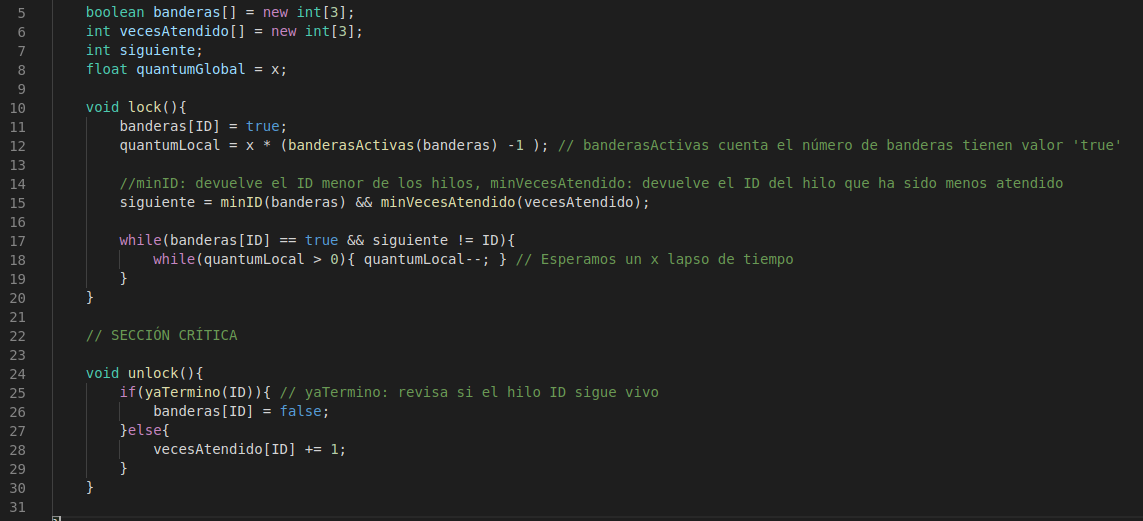
\includegraphics[width=\textwidth]{EM}\\
\begin{itemize}
\item[a) ] Demuestra que cumple con la propiedad de exclusión.
[Por Contradicción.]

Sean A, B y C, supongamos que el valor de ID es menor consecuentemente.
Supongamos que existe una ejecución $CS_A \nrightarrow CS_B$ y $CS_B \nrightarrow CS_A$.
para cualesquiera dos procesos. Tenemos dos casos dado el algoritmo para que esto suceda:
\begin{itemize}
\item[Caso a. ] Tienene diferente cantidad de veces atendidos. Supongamos que A ha sido atendido menos veces.\\
Primero ocurrió que:
\[1a)write_A(banderas[A] = true)\] \[ \rightarrow write_A(siguiente = (minID\hspace{0.2cm}AND \hspace{0.2cm}minVecesAtendido) = A)\]
Para que A entre a la sección crítica:
\[1b) read_A(banderas[A] == true)\hspace{0.2cm}AND\hspace{0.2cm}read_A(siguiente == A) \rightarrow CS_A\]
Además, primero ocurrió que:
\[2a)write_B(banderas[B] = true)\] \[ \rightarrow write_B(siguiente = (minID\hspace{0.2cm}AND \hspace{0.2cm}minVecesAtendido) = A)\]
Para que B entre a la sección crítica:
\[2b) read_B(banderas[B] == true)\hspace{0.2cm}AND\hspace{0.2cm}read_B(siguiente == B) \rightarrow CS_B\]

Por lo que hay una contradicción entre 2a y 2b ya que la varibale "siguiente" fue escrita con el valor de "A" pero B leyó que el siguiente era "B"

\item[Caso b. ] Tienen la misma cantidad de veces atendidos.\\

De manera análoga al caso anterior, suponiendo las misma condiciones. El valor que leería B en la variable "siguiente" es "B" para entrar en sus sección crítica, pero por el valor léxcio de A, es menor que B (o C), por lo que la varibale A sería escrita con el valor de "A" y de esta manera B no podría leer "B" si en la última escritura de "siguiente" fue "A".

\end{itemize} 
\item[b) ] ¿Es libre de deadlock?\\

Sí, ya que por el valor que se necesita para dejar de estar bloqueado, es del valor de los ID de cada hilo, estos ID's son únicos y en algún momento pasará debido a que se van atendiendo a los procesos según su cantidad de veces que se antendieron y el valor de su ID, por lo que no importa si tienen el mismo valor en atenciones se desempatará por el valor de su ID que es único.

\item[c) ] ¿Es libre de hambruna?\\

Sí ya que como es con base en un 'quantum' especificado, cada uno irá siendo atendido en determinado tiempo, y junto con su atención de cada proceso según el valor de su ID, estos irán siendo atendidos al menos en una ocasión.

\end{itemize}



\item[8. ] Eres uno de los $P$ prisioneros arrestados recientemente, pero el guardia de la carcel quiere darles una oportunidad para salvarse. Él ordenará a todos los prisioneros en una línea, y colocará sombreros de color rojo o azul en sus cabezas. Ningún prisionero conoce el color de su propio sombrero o el color de cualquier sombrero detrás de él, pero si puede ver los sombreros de los prisisoneros que están en frente. El guardia comenzará desde el final de la línea y pregunta a cada prisionero el color de su propio sombrero, el cual solo puede responder rojo o azul. Si da con la respuesta incorrecta será aventado a los cocodrilos, pero si contesta corrrectamente será liberado. Cada preso puede escuchar la respuesta de los prisioneros detrás de él, pero no puede decir si ese prisionero tenía razón o no.

\begin{itemize}
\item[a) ] Diseña una estrategía para salvar al menos a $P-1$ prisioneros.
Como sabemos que solo hay dos colores $Rojo$ y $Azul$, los prisioneros se pondrán de acuerdo para elegir un color y dar la clave sobre este. Supongamos que eligen el color $Rojo$. Entonces el primer prisionero que responde (el de hasta atrás) verá la cantidad de sombreros rojos, si el número de sombreros rojos es par, el prisionero responderá $"Rojo"$, si el color de sombreros rojos es impar entonces el prisionero responderá $"Azul"$, entonces todos sabrán desde un inicio si el número de sombreros rojos es par o impar. Supongamos que el último prisionero dice $Rojo$, entonces sabrán que hay un número par de sombreros rojos. Para los primeros que vean un número par de sombreros rojos sin haber escuchado previamente que alguien respondierá rojo, entonces sabrán que su sombrero es azul, el primer prisionero que vea una cantidad impar de sombreros sabrá que su sombrero es rojo, pues el hace la cantidad par de sombreros. Después de él, todos sabrán que ya hay una cantidad impar de sombreros rojos, por lo que todos los siguientes que vean una cantidad impar sabrán que tienen un sombrero azul, el primero que vea una cantidad par de sombreros sabrá que el tiene el sombrero rojo que hace la cantidad par. Y así sucecivamente.

Ahora, si desde un inicio el primer prisionero dice $"Azul"$, sabrán todos que hay una cantidad impar de sobreros rojos, por lo que el primero que vea una cantidad par de sombreros, sabrá que su sombrero es el que forma la cantidad par, cambiando ahora la cantidad de rojos a par, y todos los que vean una cantidad par o impar según la cantidad actual que hay de sombreros rojos sabrán que tienen un sombrero azul. Y así sucesivamente.

Por lo que deben fijar un color desde el principio, y dirán si el color fijado si el primer prisionero ve una cantidad par de este o el color contrario si ve una cantidad impar del color fijado.
\item[b) ] Supón que ahora el guardia puede utilizar k colores. ¿Cuál sería ahora la estrategia?
\end{itemize}


\end{itemize}



\end{document}